% !TeX program = xelatex
% !TeX encoding = UTF-8
\documentclass[UTF8]{standalone}
\usepackage{amsmath,fourier,ctex,tikz}
\begin{document}
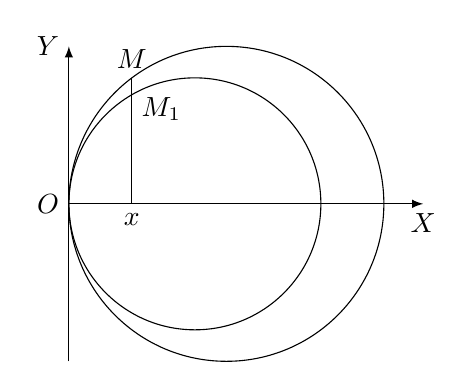
\begin{tikzpicture}
	\draw[-latex] (0,0) node[left] {$O$} -- (4.5,0) node[below] {$X$};
	\draw[-latex] (0,-2) -- (0,2) node[left] {$Y$};
	\draw (2,0) circle (2);
	\draw (1.6,0) circle (1.6);
	\draw (0.8,0) node[below] {$x$} -- ++ (0,1.6) node[above] {$M$};
	\node[right] at (0.8,1.2) {$M_{1}$};
\end{tikzpicture}
\end{document}